%----------------------------------------------------------------------------------------
% Einführung in das Wissenschaftliche Arbeiten 
% Report LaTeX template (English)
% Interactive Graphics and Simulation Group
% University of Innsbruck
%----------------------------------------------------------------------------------------

\documentclass[11pt,a4paper]{article}

%----------------------------------------------------------------------------------------
% Include required packages
\usepackage{graphicx}
\usepackage{amsmath}
\usepackage{pdfpages}
\usepackage{url}
\usepackage{subfig}
\usepackage{fancyhdr}
\usepackage{lastpage}
\usepackage{float}
\usepackage[english]{babel}
%\usepackage[ngerman]{babel}

\usepackage{listings}
\usepackage{xcolor}
\lstset {
    backgroundcolor=\color{black!5}, % set backgroundcolor
    basicstyle=\scriptsize,% basic font setting
    captionpos=b,
    numbers = left,
    breaklines=true,
}

%\usepackage[utf8x]{inputenc}
%\usepackage[T1]{fontenc}

\usepackage[left=2.7cm, right=2.7cm, top=3cm]{geometry}

% Set up the header and footer
\pagestyle{fancy}
\rhead{}
\lhead{}
\chead{}
\lfoot{Sch{\"o}pf, Spiss} % Bottom left footer
\cfoot{Physical based simulation - Final Project} % Bottom center footer
\rfoot{Page\ \thepage\ of\ \protect\pageref{LastPage}} % Bottom right footer
\renewcommand\footrulewidth{0.4pt} % Size of the footer rule
\renewcommand{\headrulewidth}{0pt}
\setlength\parindent{0pt} % Removes all indentation from paragraphs

%----------------------------------------------------------------------------------------
% Start document

\begin{document}


%----------------------------------------------------------------------------------------
% Title page
%----------------------------------------------------------------------------------------

\begin{titlepage} % User-defined title page

\begin{center}

\includegraphics[width=1.2cm]{images/uibk}

\begin{large}
Leopold-Franzens-Universit\"at Innsbruck\\[5mm]
Institute of Computer Science\\
\end{large}

{\LARGE \bf Final Project}

Physical based simulation PS\\[20mm]

Lukas Sch\"opf\\Stefan Spiss\\[35mm]

advised by\\
M.Eng.~Oquang~Van~Ha\\[10mm]

\vfill

Innsbruck, \today
\end{center}

\end{titlepage}


%----------------------------------------------------------------------------------------
% Main body
%----------------------------------------------------------------------------------------

\section{Introduction}
\label{sec:intro}
In our final project we implemented a ball game in which the goal is to navigate a rolling ball through a maze by tilting the playing field. To implement our game we used SDL2 with OpenGL and GLM. We mainly concentrated on collisions and the rigid body model.\\
The final result graphics implementation can be seen in figure~\ref{fig:gamemaze}.
\begin{figure}[H]
\centering
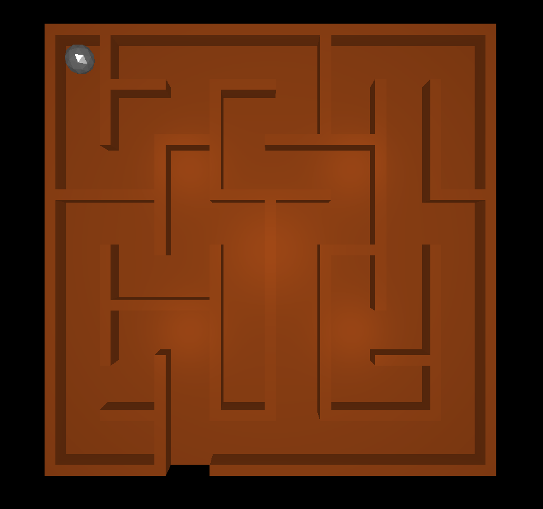
\includegraphics[width=0.5\textwidth]{images/ballmaze}
\caption{game maze}
\label{fig:gamemaze}
\end{figure}

\section{Graphics Framework}
\label{sec:graphic}
For the visualization of the game we implemented a graphics framework in C++ using the graphics library OpenGL 3.3\footnote{OpenGL: \url{https://www.opengl.org/}}, the multimedia library SDL 2.0\footnote{SDL 2.0: \url{https://www.libsdl.org/}} and the C++ mathematics library glm\footnote{glm: \url{http://glm.g-truc.net/0.9.8/index.html}}. As the generated mazes are saved as .obj files (see section~\ref{sec:mazeGeneration} for details) the open source object-file-loader tinyobjloader from Syoyo Fujita~\cite{tinyobjloader} is employed to load the mazes and the ball. Furthermore, it has to be mentioned, that the framework was implemented with the help of an old computer graphics project from Philipp Mildenberger\footnote{git repository of CG-Project, Philipp Mildenberger: \url{https://github.com/Philipp-M/CG-Project}}, which was only used as reference for some concepts of the OpenGL pipeline.

\section{Physics Model}
\label{sec:physics}
For the physics calculation and the collision detection, the maze walls and the ball were represented in an additional physics model. In the source code the related physics implementation can be found in the files: \emph{Physics.hpp and Physics.cpp} which contain the classes: \emph{Physics}, \emph{Collision}, \emph{StaticObject} and \emph{Ball}. The ball is simply described by its center point and its radius, AABB boxes represent the walls and the floor of the maze (see section~\ref{sec:collision} for details). Instead of tilting all the physical models according to the rotation of the visual maze, only the gravity vector is tilted as this results in the same effect and simplifies collision detection. In the following of this section the different used physical-based simulation methods are explained more in detail, starting with rigid bodies, which are the basis of the physics simulation in this project. After that it is explained how the rolling of the ball is implemented. Furthermore, rolling friction is described in the end of this section. 

\subsection{Rigid Body}
\label{subsec:rigid}
The object dynamics in this project are calculated using rigid body simulation. In this method it is assumed, that all objects are incompressible and the dynamic state of each object is given by its translation and rotation. 
%Furthermore, when using random objects, each object has many mass points and the center of mass is somewhere in the middle of the object with the condition that all the object mass points
Because of the chosen physics ball model, it is very simple to calculate the rigid body dynamics update step. Additionally, the walls and the floor of the maze are assumed to be static and therefore are approximated as rigid bodies with infinite mass. In the beginning of a rigid body simulation, all the objects have to be initialized, according to the lecture slides \emph{Physically-Based Simulation Rigid Bodies 1}, pages 31 and 32. For the initialization of the ball, only the inverse inertial tensor has to be obtained as the total mass, the mass center and the radius are given. The inverse inertial tensor is calculated as following:

$$I^{-1} = \frac{5}{2mR^2}\begin{pmatrix}
1 & 0 & 0 \\ 
0 & 1 & 0 \\ 
0 & 0 & 1
\end{pmatrix}$$

Additionally, the initial velocity $v$, angular momentum $L$ and rotational velocity $\omega$ are set to zero and the rotation matrix $A$ is initialized as identity.

The whole update step for the rigid body is calculated using a Symplectic Euler step. At first, all the forces $f$ acting on the ball are computed. In our case, for that only the earth acceleraction and the ball friction have to be considered, which results in the following force calculation:
$$f_{t} = g_{vec3} \cdot m + f_{roll_friction}$$
Then the velocity is obtained as follows:
$$v_{t+dt} = v_{t} + dt \cdot \frac{f_{t}}{m}$$
And after that, only the center point position of the ball has to be update according to:
$$x_{t+dt} = x_{t} + v_{t+dt} \cdot dt$$

The rigid body model also includes methods to handle torque angular momentum and rotation. These aren't explained here because our physics model isn't influenced by these methods. We opted to implement the rolling of the ball via approximations, as applying torque to the ball in a physically correct way via the rigid body model proves to be difficult. A full description of the rigid body model can be found in the lecuture slides: Sim08\_Rigid+Bodies+1\_WS16.pdf.

\subsection{Rolling Ball}
\label{subsec:rollingBall}
As it is more complex to simulate a rolling ball using collisions with the floor to influence the inertial moment. We chose to reduce the acting force according to the rolling inertia of the Ball.
This can be explained as follows. Basically a rolling ball "stores" energy in the rotation. This can be seen as a reduction of the outside force acting upon it. 
$$E_{tot} = E_{kin}+E_{rot}$$
$$E_{tot} = \frac{m v^2}{2} +\frac{I\omega^2}{2} $$ 
substitute I for a filled ball and for non slip rolling
$$I=\frac{2mR^2}{5} \omega = \frac{v}{R}$$
approximate gained total energy as potential energy $mgh$
$$ mgh =  \frac{mv^2}{2}+\frac{mv^2}{5}$$
solve for $v$
rolling:
$$v=\sqrt[]{\frac{7}{5}gh}$$
non rolling:
$$v=\sqrt[]{2gh}$$
From this we can see, that decreasing the acceleration has the same effect on the ball movement as calculating the inertial tensor. 
\\
For the optical effect of the ball rolling we used the simple relation between the rotation speed $\omega$ the radius $r$ and the velocity $v$.
$$\omega = \frac{v}{r} $$
With this we can directly calculate the rotation of the ball via the velocity and update the rotation of the ball in the graphics model accordingly.


\subsection{Rolling Friction}
\label{subsec:rollingFriction}
To calculate the friction force $F_r$ of our rolling ball we use the equation:
$$F_r=\mu F_N$$
Whereas $F_N$ is the normal force on the surface. In our case this is just the z-component of the gravity acceleration vector, as the vector is tilted to move the ball instead of the playing field.
$\mu$ is the friction coefficient which describes how much rolling resistance there is between the ball and the surface. A typical value for a scenario similar what we are simulating (a metal ball on wooden floor) is 0.003. This friction force has to be applied in the opposite direction of the movement vector if the velocity is greater than zero. In the resting case the rolling fricition inhibits the ball from moving if the force moving the ball is smaller than the rolling friction force.

\section{Collision Detection}
\label{sec:collision}
For collision detection in this project we use AABB bounding boxes as borders and detect collisions between the sphere and the bounding boxes. As the shortest distance calculation between the sphere and the AABB box is very compute efficient and we don't have many bounding boxes in our labyrinth we check for collisions with every box on the playing field every iteration. For a future improvement one could just include the boxes in proximity to the ball depending on the maximum velocity.

To calculate the distance between the AABB bounding box and a point we only need to check each axis.
In the example in figure~\ref{fig:AABB} the points x coordinate is first checked if it is smaller or larger than the min or max point defining the AABB box. If it is in between we choose the spheres center point x coordinate for the point on the surface we calculate the minimum distance to.
The same is done for the y coordinate of the center point, where the minimum points y coordinate is set. If we now calculate the distance between the centerpoint and our calculated point on the surface and check if it is smaller than the radius of our sphere we can decide if a collision has happened or not. For reflecting the ball on a surface the surface normal is also important. The surface normal can be calculated by subtracting our calculated point from the spheres center. For the 3D case, as we use it in our project, we can simply expand this method with the z-axis.

%In figure~\ref{fig:AABB} different cases of our fluid simulation can be seen.
\begin{figure}[H]
\centering
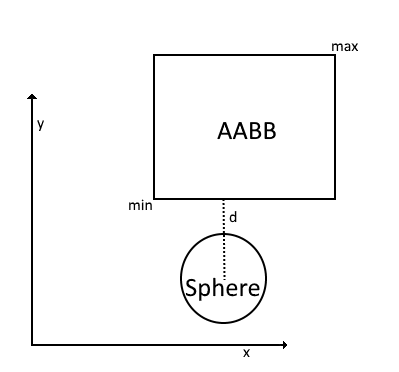
\includegraphics[width=0.5\textwidth]{images/AABB}
\caption{AABB collision detection}
\label{fig:AABB}
\end{figure}


\subsection{Collision Steps}
\label{subsec:collisionSteps}

Once a collision is detected the ball is moved outside of the bounding box along the surface normal, so the distance between the balls center point and the bounding box equals the radius. This is not 100\% correct and results in a small error, but due to the small time step for the physics simulation(10 ms) this is negligible in our implementation. Because of this we also don't need to look out for the ball moving through the borders in one update step.
The next step is to update the velocity according to the rigid body model.
For this the impulse magnitude $j$ is calculated first:
$$j=\frac{-(\epsilon+1)\cdot v_{ball}^{t-}\boldsymbol{n}}{\boldsymbol{nn}m_{ball}^{-1}}$$
Then the velocity is updated according to:
$$v_{ball}^{t+} = v_{ball}^{t-}+ \frac{j \cdot \boldsymbol{n} }{m_{ball}}  $$

\newpage
\section{Maze Generation}
\label{sec:mazeGeneration}
As only having a single maze(level) in the game would be boring we used a python script to generate random mazes\footnote{maze generator: \url{http://www.thingiverse.com/thing:24604}}.
This script generates openscad files by default. To be able to get the AABB collision box boundaries from the maze generator the script was modified to output a .txt file which can be loaded from our program. Because OpenScad can only generate .stl files and not .obj files blender had to be used to convert the OpenSCAD output to .obj to be compatible with the tinyobj loader. The workflow to generate a new maze is as follows: 

\begin{itemize}
	\item run python script to generate .scad file and AABB bounding box coordinates
	\item run OpenSCAD to generate a .stl file
	\item run blender to generate a .obj file from the .stl file
	\item replace default material file definitions to match the desired visual properties
\end{itemize}

The whole process of generating a maze is rather compute intense due to the cad programs involved and thus takes a long time($>10$ seconds) to complete. Because of this we decided to pre generate different mazes and load these in our game once a level is completed. In the current implementation 10 different mazes are used which can be generated in advance using the bash script generatemaze in the folder Maze\_Generation. For this to work OpenSCAD and Blender need to be installed on the target machine. The default cube in blender needs to be disabled as described in: \url{http://blender.stackexchange.com/questions/5574/how-to-remove-the-default-cube}.


\section{System Overview}
\label{sec:systemOverview}
The program is divided into two parts, one does the physics calculation in a seperate thread with a higer update rate and the other displays the current graphics state via OpenGL. The 

\section{Conclusion}
\label{sec:conclusion}
All in all this was an interesting and challenging project. Setting up the graphics framework in the beginning turned to be one of the most challenging parts. We also put some thought into how to make the ball roll realistically. In the beginning we implemented the full ridgid body model including all angular components. Calculating the torque from the friction with the surface proved to be non-trivial, thus without torque the angular components from the rigid body model are not affected. Thus we approximated the simulation of the rolling ball via other means. We also had problems with continuous collisions becoming unstable. Decreasing $\epsilon$ (an $\epsilon < 1$ results in energy being dissipated during a collision) in the j term and changing the forward euler method to the energy conserving symplectic euler method improved stability.
%----------------------------------------------------------------------------------------
% Bibliography
%----------------------------------------------------------------------------------------
\newpage
\bibliographystyle{plain}
\bibliography{biblio_physical_based_simulation}


\end{document}
